\chapter{Results}
\todo{Lav systematiske resultater. Udvælg functionsklasser at kigge på}

<reproducer resultater fra Arayns thesis>
Egne forsøg med SPN og mixture regression


\section{implementation}
The Gaussian process regression is implemented using the Scikit-learn Gaussian process
implementation with the Matern kernel with $\nu=1.5$ and the y-values are normalized in order for
the prior distribution to be reasonable (mean 0 and variance 1). The lengthscale is optimized by
maximizing the marginalized likelihood using the limited memory quasi newton solver with bounds
l-bfgs-b with 200 restarts. 

The Bayesian neural network is implemented using Numpyro - which is a python library for
probabilistic machine learning, developed by some of the people behind Pyro, but instead of using
pyTorch as backend, Numpyro uses Jax. This allows for significantly large speedup when doing MCMC,
i.e. NUTS sampling. This was however still very slow and we therefore limited the network size to a
small 3 layer with 10 nodes on each layer network. The prior distribution for weights is a standard
normal distribution, and the bias normal priors are sat 
a bit less restrictive with a standard deviation of 2 instead. 
This is reasonable since the data is always standardized. 

\subsection{standardized data}
Before the data reach any of the models, it is standardized. Which is 
a scaling and translation such that the datas empirical mean and standard deviation are 0 and 1, respectively. 
In that way is much easier to control the parameters in the models, since the data it fits and predicts
is always the same scale. The transformation is as following, first time the models sees the data, 
the empirical mean and standard deviation is recorded both for $x$ and $y$, (note $x$ can be a vector),
giving $\mu_x$,$\mu_y$, $\sigma_x$and $\sigma_y$.
next all data is transformed using the transformation, 

$$T_x(\cdot) := \frac{\cdot-\mu_x}{\sigma_x}$$

When we predict the $x$ is transformed, the model output a prediction 
and then the inverse transform is mapping the prediction from the standardised
domain to the original domain, 
 $T^{-1}_y(\hat y) := \hat y \cdot \sigma_x+\mu_x$


\section{Regression analysis}
As described in the previous sections an essential part of Bayesian optimization and the decision theory build 
around Bayesian optimization, that the regression model is correct. We will therefore look at how good the
regression models are, both in terms of correct prediction and in terms of correct uncertainty estimation. 

\subsection{uncertainty quantification}
The probibalistic model is given as 
$$p(y|x,\mathcal{D}) = \mathcal{N}(y|\mu_{\mathcal{D}}(x), \sigma_{\mathcal{D}}^2(x))$$
where the mean, and variance functions are different for all the models. 
Given a trained model, we quantify its ability to capture uncertainty with the average
predictive likelihood/ probability of the observation, given a test input $x_i$ the
the density of predictive distribution is evaluated in the coresponding test output $y_i$,

$$\overline{p(y_i|x_i,\mathcal{D})} := \frac{1}{n}\sum_{i=1}^n p(y_i|x_i,\mathcal{D})$$
there the bigger the mean predictive likelihood is, the better. \todo{it is not called preditive
likelihood!!}

\subsection{prediction quantification}
Here we use the mean absolute error to quantify the prediction error. The i'th test point is
$(x_i,y_i)$ and the mean absolute error is given as, 
$MAE :=\frac{1}{n}\sum_{i=1}^n |\mu_{\mathcal{D}}(x_i) - y_i| $

\subsection{regression benchmark}
We will benchmark our different regression models againt a simple emperical mean and
emperical std. normal distribution benchmark, 
$$p(y|x\mathcal{D}) = \mathcal{N}(y| \bar{\textbf{y}} , \bar{\sigma}^2 (\textbf{y}))$$

where $\bar{\textbf{y}} = \frac{1}{n}\sum_{i=1}^n \textbf{y}_i $ and 
$\bar{\sigma}^2 (\textbf{y})) = \frac{1}{n-1}\sum_{i=1}^n (\textbf{y}_i-\bar{\textbf{y}})^2 $
this is however not a good model for Bayesian optimization, as it will not provide a
new candidate point, as all points are equally good. 


\section{Mixture regression}

\begin{figure}
  \caption{Regression of a probabilistic objective function, is not a smart choice
  using anything else than a mixture regression model. Top we see the performance
  of 5 different regression models fitted to an increasing amount of training data, 
  the underlying function is tricky, as it jumps between multiple objective functions
  yielding a violation to most of the generative models, where most are capable of
  handling gaussian noise this is not gaussian noise and hence a very difficult problem. 
  This kind of objective function could definitely be relevant in certain cases.}
\end{figure}

One could define a generative story, flip a coin, then the data will
be fitted with this Gaussian.! 

\begin{figure}
  \caption{Plots visulising the results in above figure.}
\end{figure}

<data generating process>
Model do well when they are the data generating process, but if they are not, then
they do bad. If you collect all model, 

What model to chose? the standard answer of a Bayesian should be: Why choose? If there 
is uncertainty about them, then we can just average them. Pic the maximum would be frquencialistic.

Could we combine GP and SPN?

ensample of models ..
Simulation studies. 


\section{Regression analysis of GP, BOHAMIANN and NumpyNN 1D}

\section{Regression analysis of GP, BOHAMIANN and NumpyNN 2D}

\begin{figure}[h]
  \centering
  \begin{minipage}[b]{0.49\textwidth}
   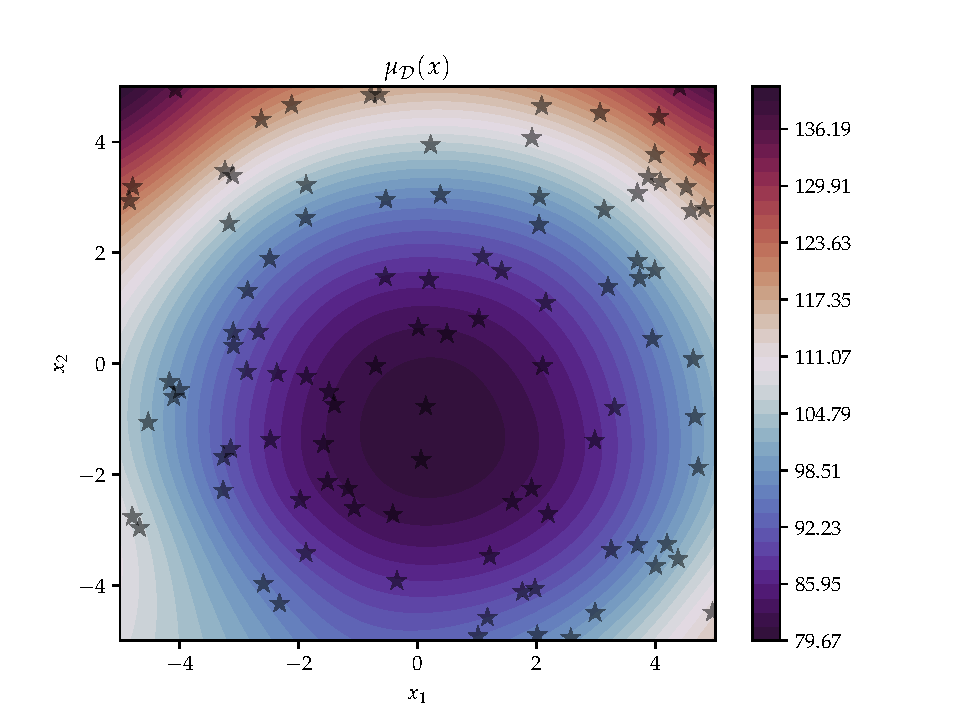
\includegraphics[trim=1.2cm 0.7cm 2cm 1cm,clip,width=\textwidth]{Figures/coco_reg/f1_BOHAMIANN2.pdf}
  \end{minipage}
  \hfill
  \begin{minipage}[b]{0.49\textwidth}
    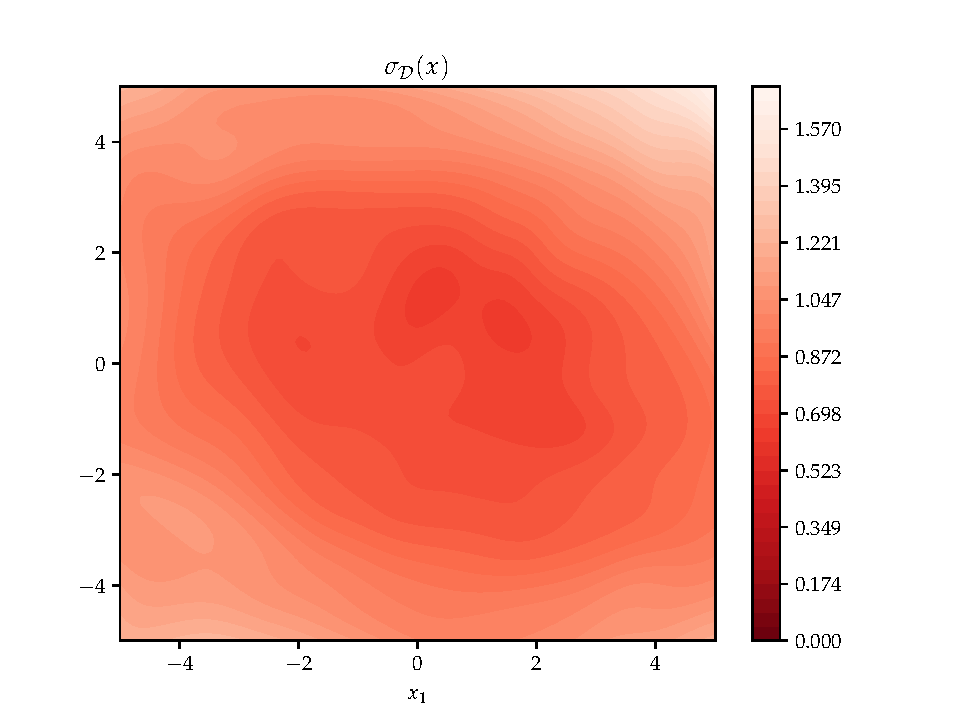
\includegraphics[trim=1.2cm 0.7cm 2cm 1cm,clip,width=\textwidth]{Figures/coco_reg/f1_BOHAMIANN3.pdf}
   \end{minipage}
  
   \begin{minipage}[b]{0.49\textwidth}
    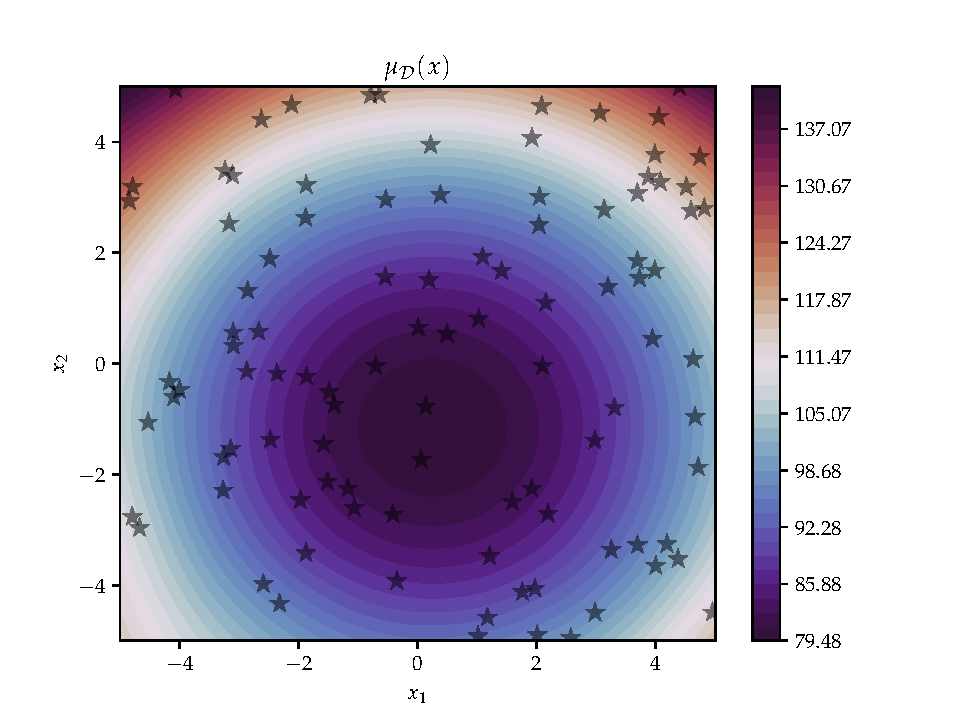
\includegraphics[trim=1.2cm 0.7cm 2cm 1cm,clip,width=\textwidth]{Figures/coco_reg/f1_Gaussian Process - sklearn2.pdf}
   \end{minipage}
   \hfill
   \begin{minipage}[b]{0.49\textwidth}
     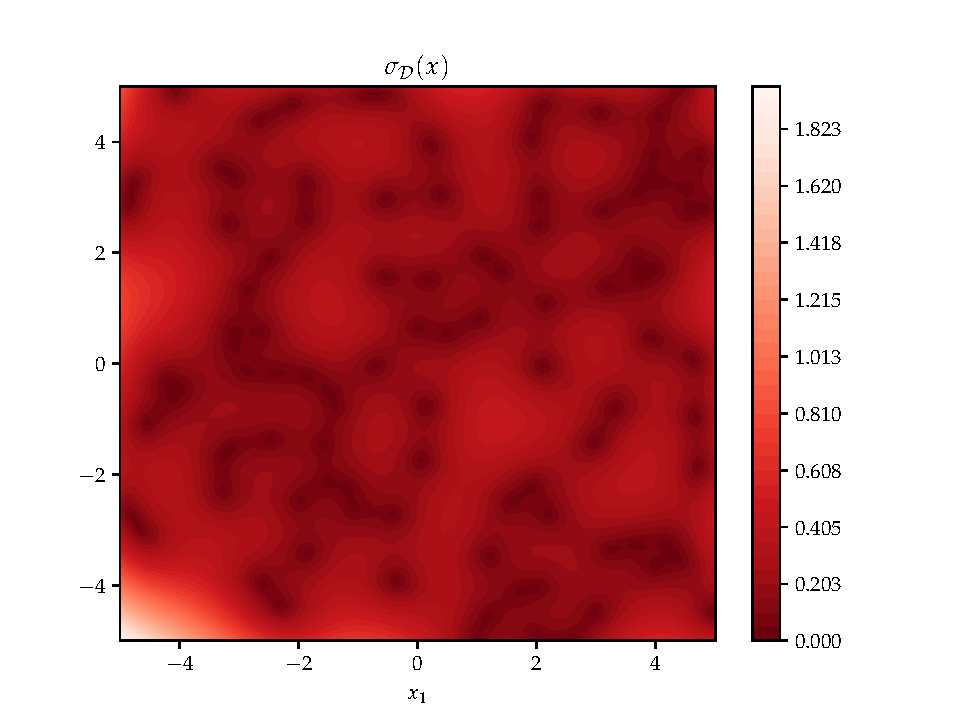
\includegraphics[trim=1.2cm 0.7cm 2cm 1cm,clip,width=\textwidth]{Figures/coco_reg/f1_Gaussian Process - sklearn3.pdf}
    \end{minipage}

    \begin{minipage}[b]{0.49\textwidth}
      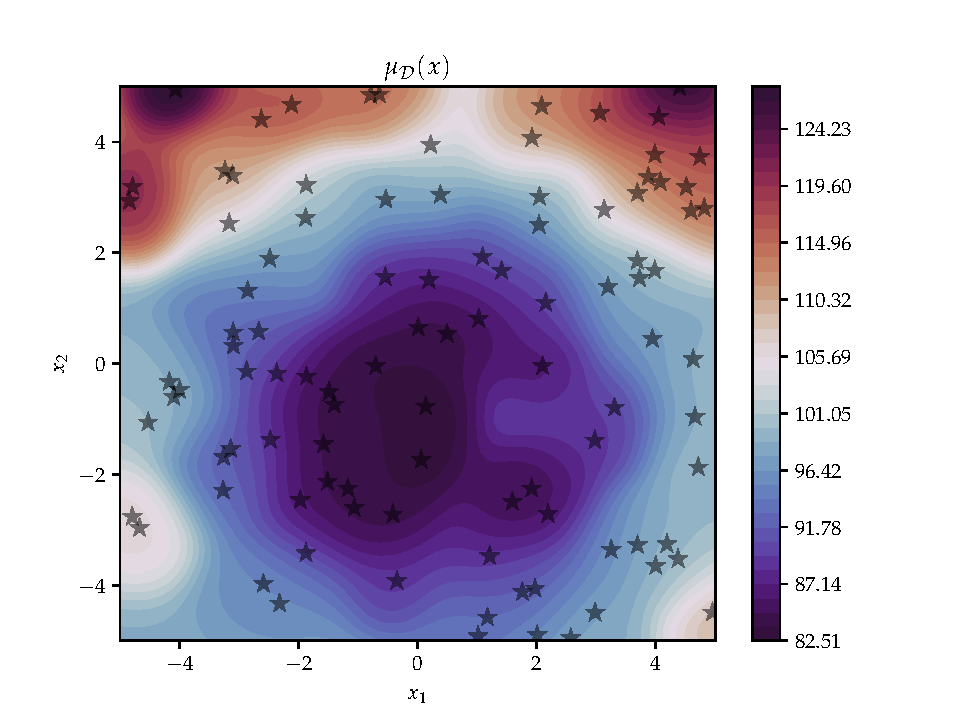
\includegraphics[trim=1.2cm 0.7cm 2cm 1cm,clip,width=\textwidth]{Figures/coco_reg/f1_Naive Gaussian Mixture Regression optimized2.pdf}
     \end{minipage}
     \hfill
     \begin{minipage}[b]{0.49\textwidth}
       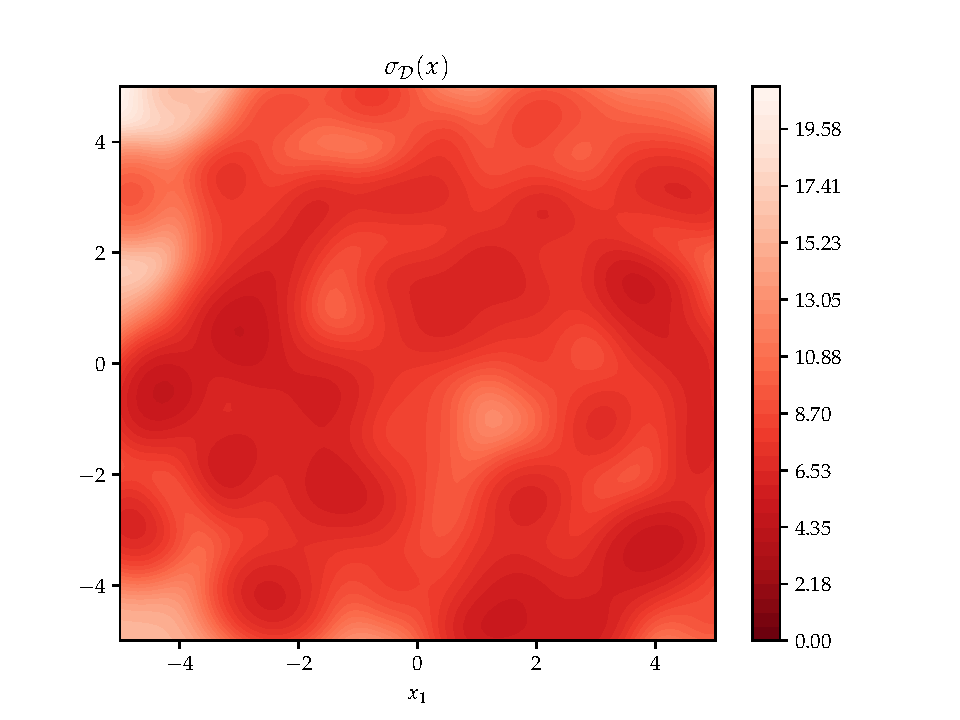
\includegraphics[trim=1.2cm 0.7cm 2cm 1cm,clip,width=\textwidth]{Figures/coco_reg/f1_Naive Gaussian Mixture Regression optimized3.pdf}
    \end{minipage}
  \label{f1_reg_2D}
\end{figure}

\begin{figure}[h]
  \centering
  \begin{minipage}[b]{0.49\textwidth}
   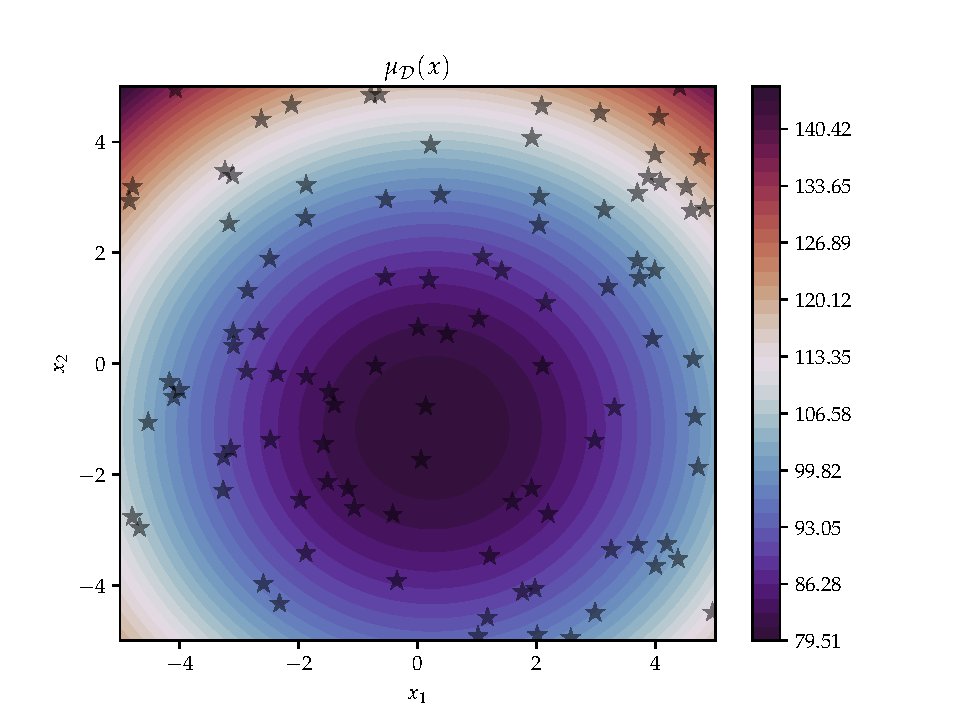
\includegraphics[trim=1.2cm 0.7cm 2cm 1cm,clip,width=\textwidth]{Figures/coco_reg/f1_numpyro neural network200-2002.pdf}
  \end{minipage}
  \hfill
  \begin{minipage}[b]{0.49\textwidth}
    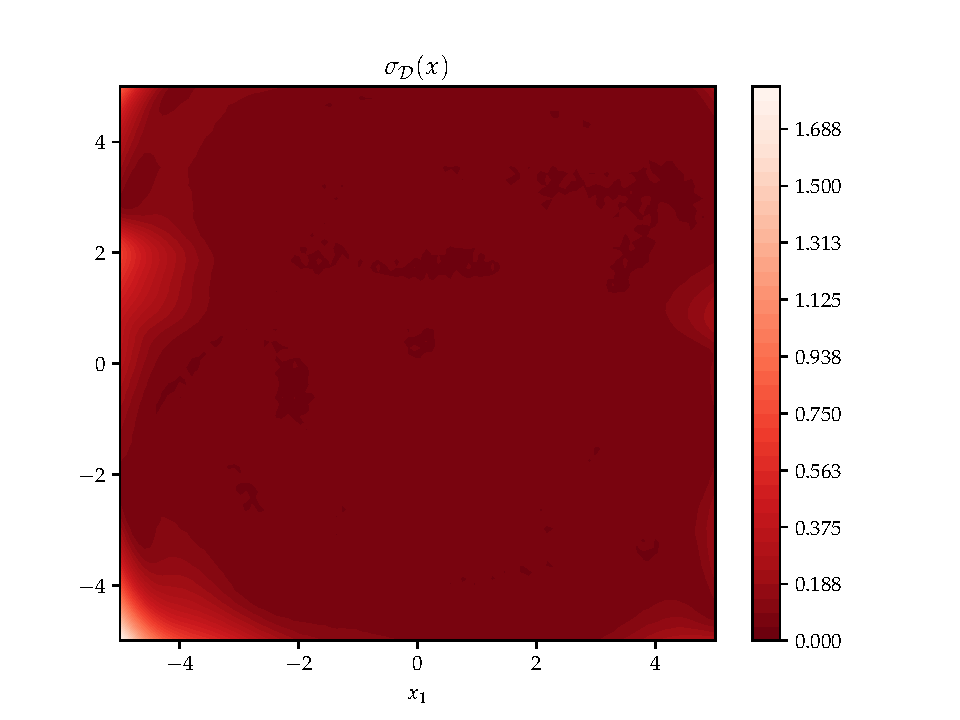
\includegraphics[trim=1.2cm 0.7cm 2cm 1cm,clip,width=\textwidth]{Figures/coco_reg/f1_numpyro neural network200-2003.pdf}
   \end{minipage}
  
  %  \begin{minipage}[b]{0.49\textwidth}
  %   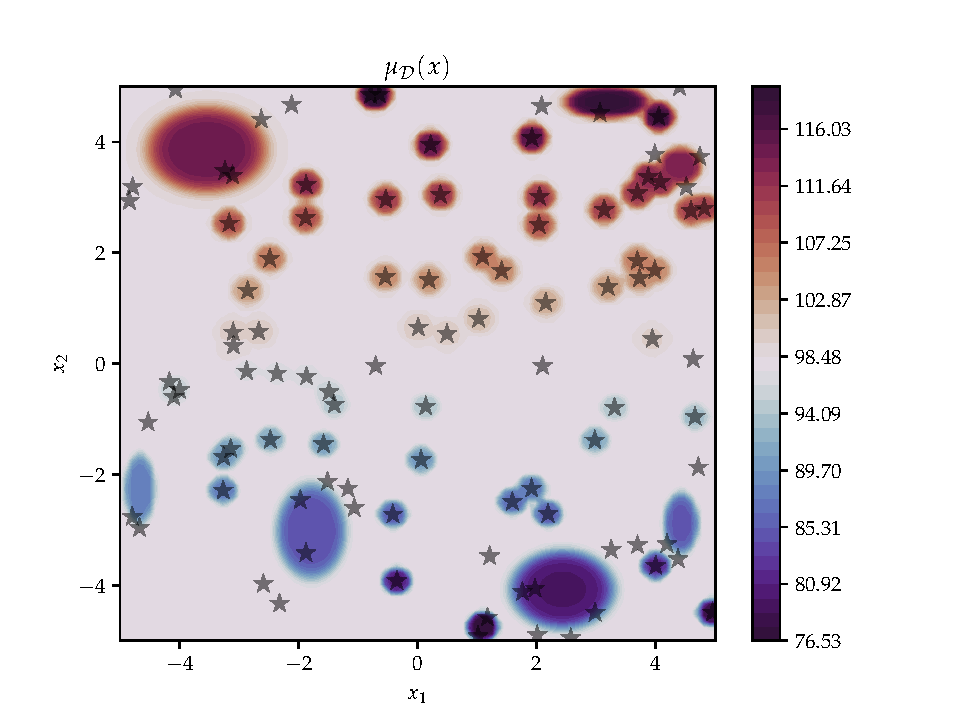
\includegraphics[trim=1.2cm 0.7cm 2cm 1cm,clip,width=\textwidth]{Figures/coco_reg/f1_SPN regression optimized2.pdf}
  %  \end{minipage}
  %  \hfill
  %  \begin{minipage}[b]{0.49\textwidth}
  %    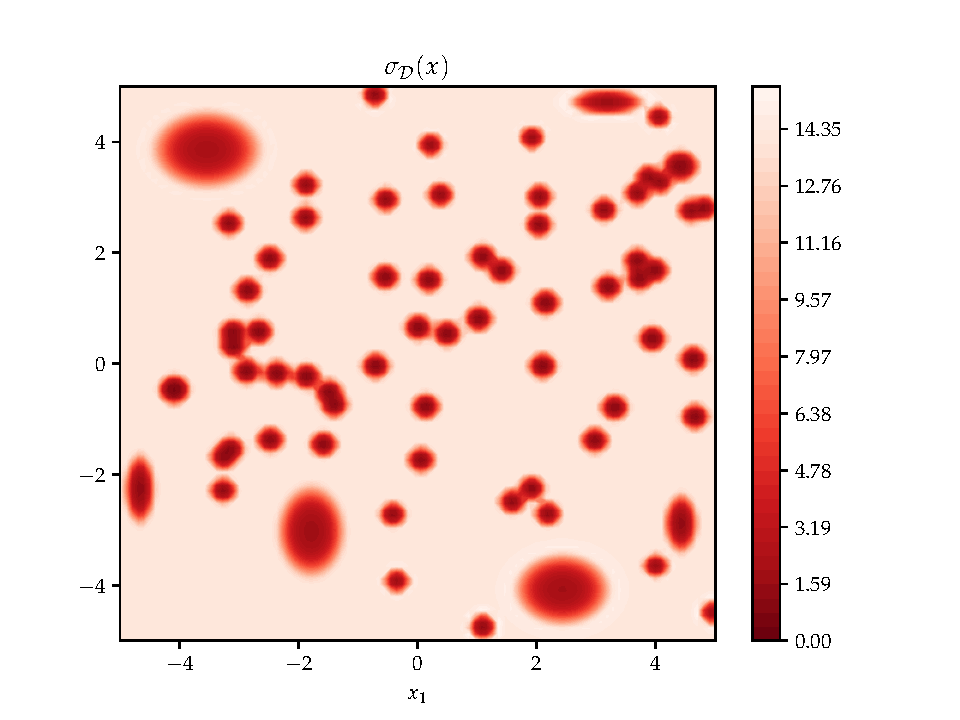
\includegraphics[trim=1.2cm 0.7cm 2cm 1cm,clip,width=\textwidth]{Figures/coco_reg/f1_SPN regression optimized3.pdf}
  %   \end{minipage}

    \begin{minipage}[b]{0.49\textwidth}
      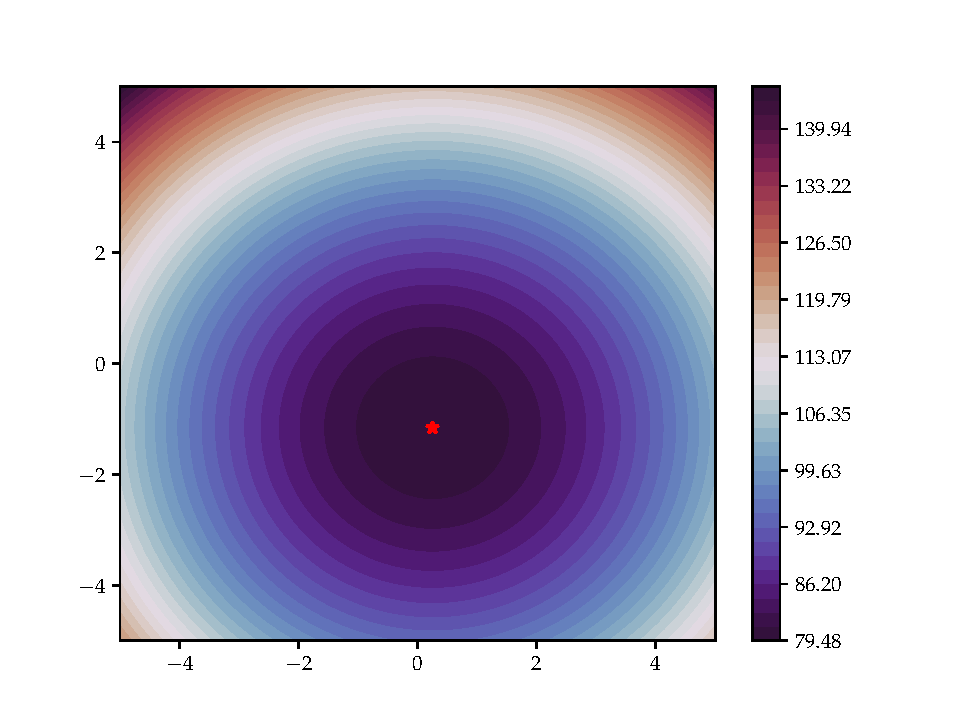
\includegraphics[trim=1.2cm 0.7cm 2cm 1cm,clip,width=\textwidth]{Figures/coco/f1.pdf}
     \end{minipage}
     \hfill
  \label{f1_reg_2D}
\end{figure}

\begin{figure}[h]
  \centering
  \begin{minipage}[b]{0.49\textwidth}
   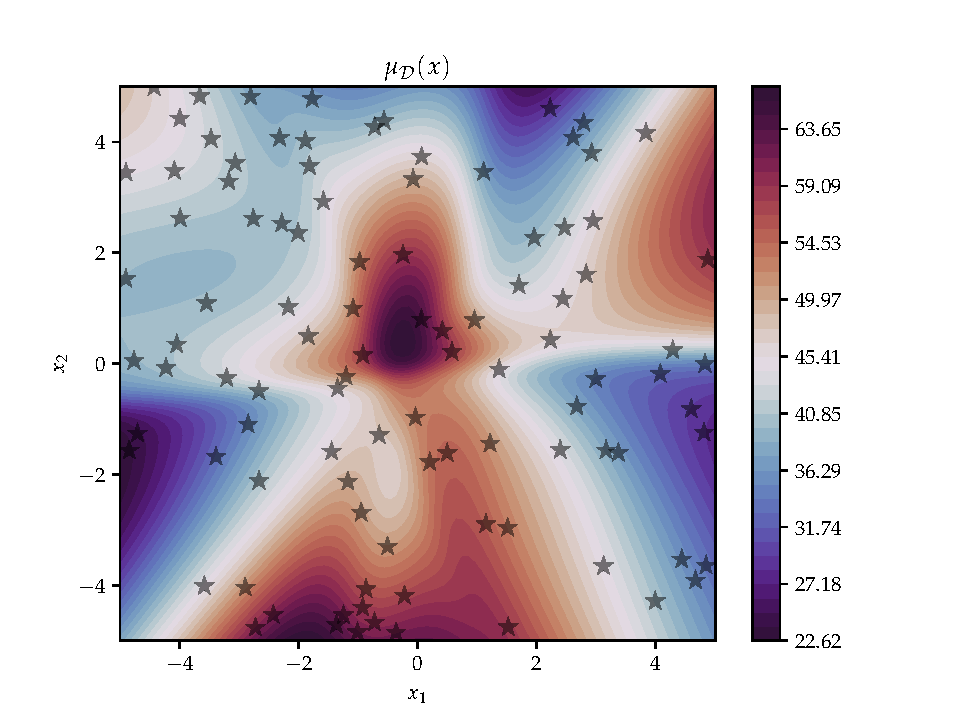
\includegraphics[trim=1.2cm 0.7cm 2cm 1cm,clip,width=\textwidth]{Figures/coco_reg/f23_BOHAMIANN2.pdf}
  \end{minipage}
  \hfill
  \begin{minipage}[b]{0.49\textwidth}
    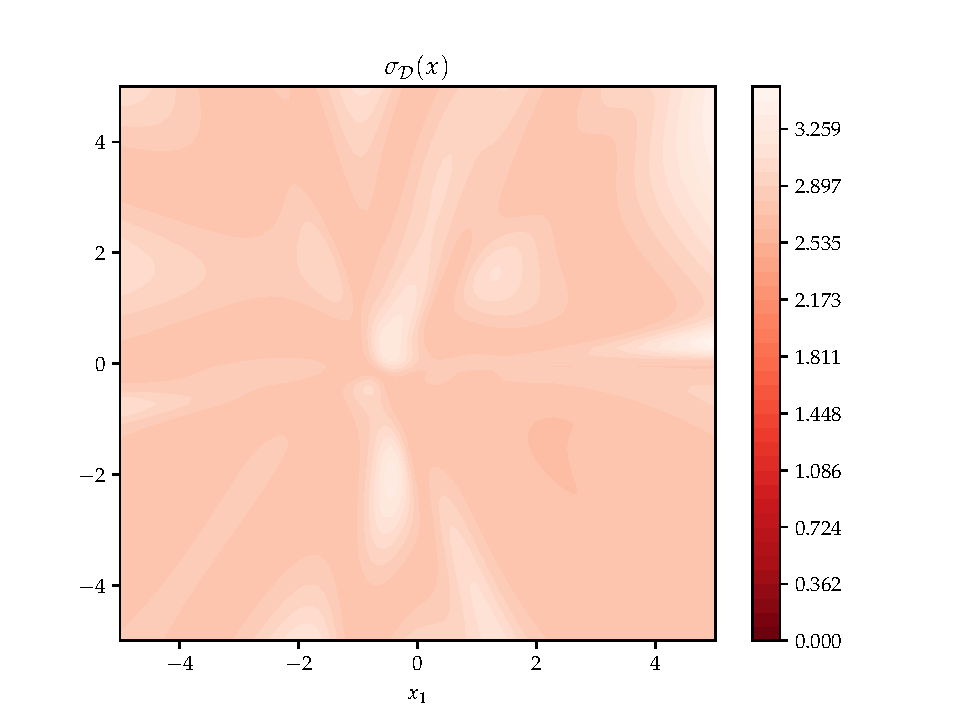
\includegraphics[trim=1.2cm 0.7cm 2cm 1cm,clip,width=\textwidth]{Figures/coco_reg/f23_BOHAMIANN3.pdf}
   \end{minipage}
  
   \begin{minipage}[b]{0.49\textwidth}
    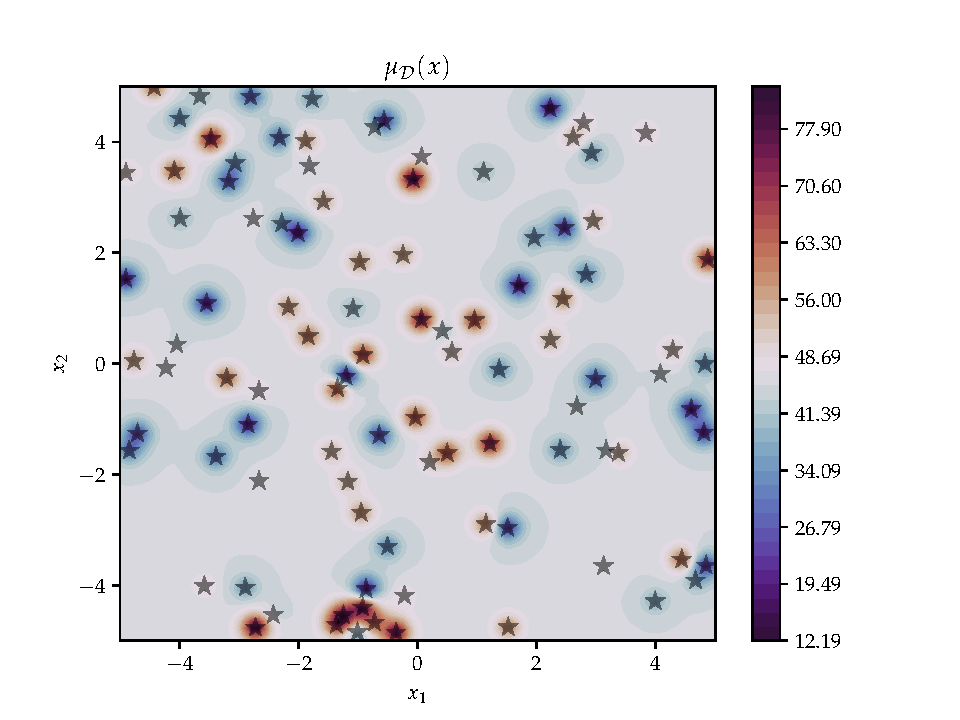
\includegraphics[trim=1.2cm 0.7cm 2cm 1cm,clip,width=\textwidth]{Figures/coco_reg/f23_Gaussian Process - sklearn2.pdf}
   \end{minipage}
   \hfill
   \begin{minipage}[b]{0.49\textwidth}
     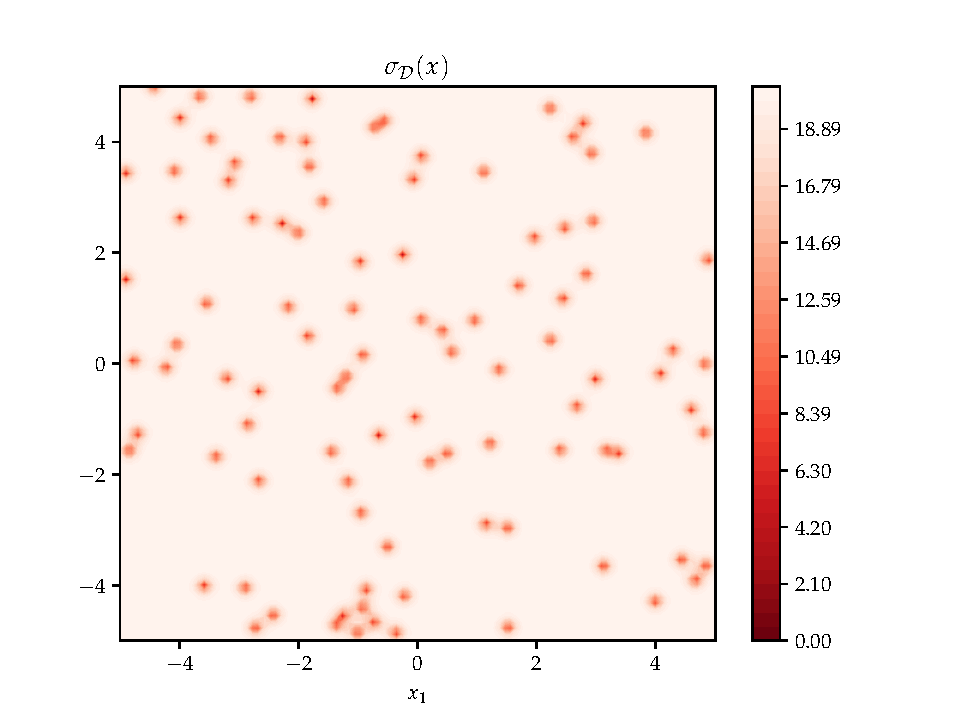
\includegraphics[trim=1.2cm 0.7cm 2cm 1cm,clip,width=\textwidth]{Figures/coco_reg/f23_Gaussian Process - sklearn3.pdf}
    \end{minipage}

    \begin{minipage}[b]{0.49\textwidth}
      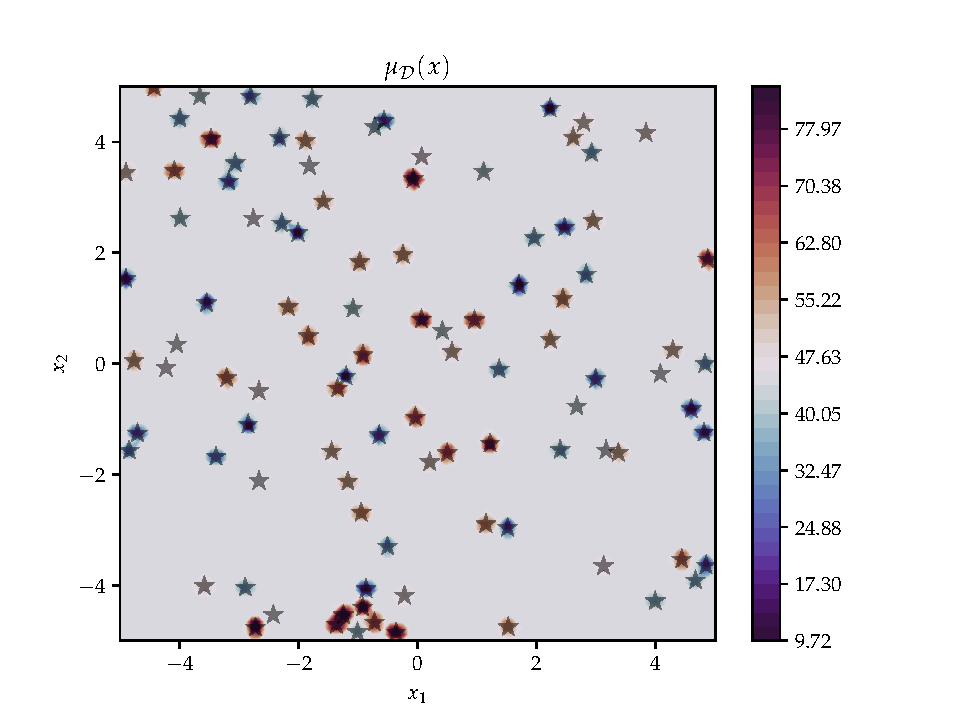
\includegraphics[trim=1.2cm 0.7cm 2cm 1cm,clip,width=\textwidth]{Figures/coco_reg/f23_Naive Gaussian Mixture Regression optimized-prior 12.pdf}
     \end{minipage}
     \hfill
     \begin{minipage}[b]{0.49\textwidth}
       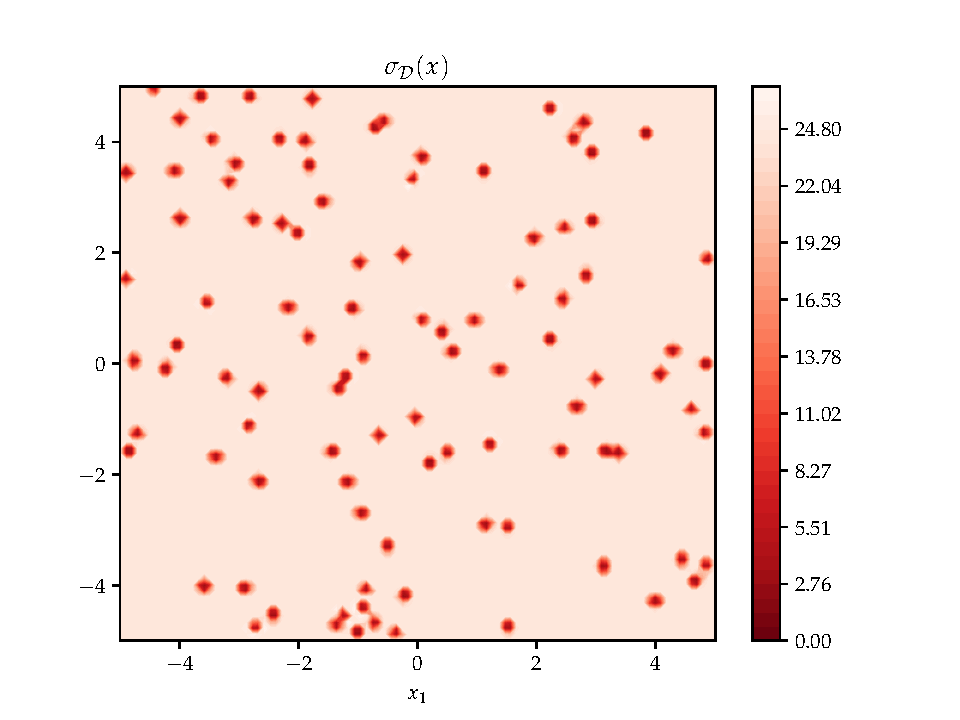
\includegraphics[trim=1.2cm 0.7cm 2cm 1cm,clip,width=\textwidth]{Figures/coco_reg/f23_Naive Gaussian Mixture Regression optimized-prior 13.pdf}
    \end{minipage}
  \label{f23_reg_2D}
\end{figure}

\begin{figure}[h]
  \centering
  \begin{minipage}[b]{0.49\textwidth}
   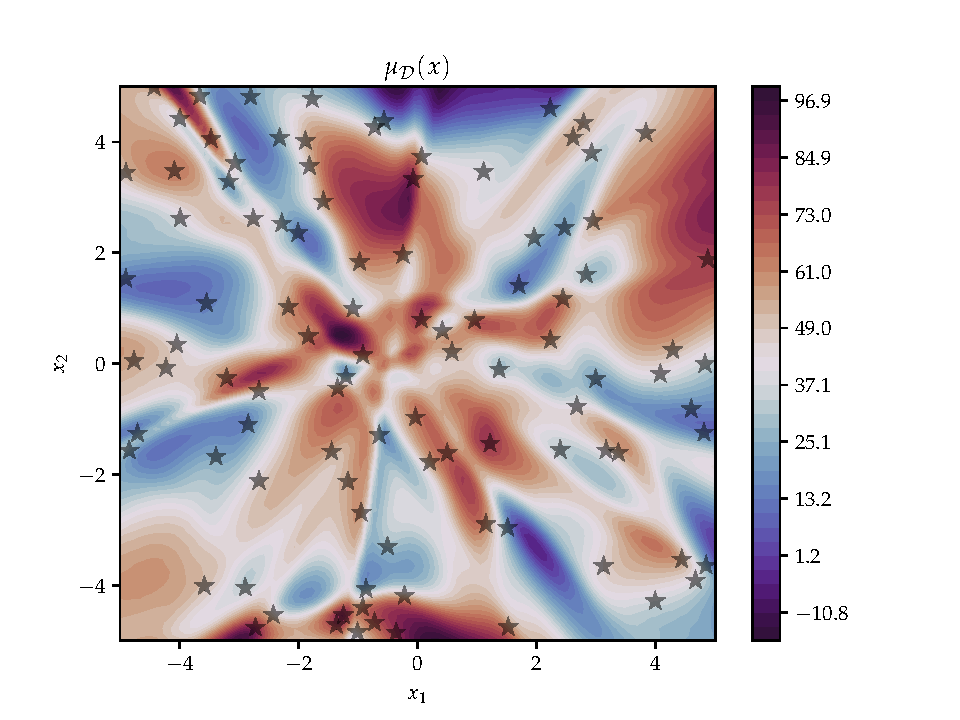
\includegraphics[trim=1.2cm 0.7cm 2cm 1cm,clip,width=\textwidth]{Figures/coco_reg/f23_numpyro neural network200-2002.pdf}
  \end{minipage}
  \hfill
  \begin{minipage}[b]{0.49\textwidth}
    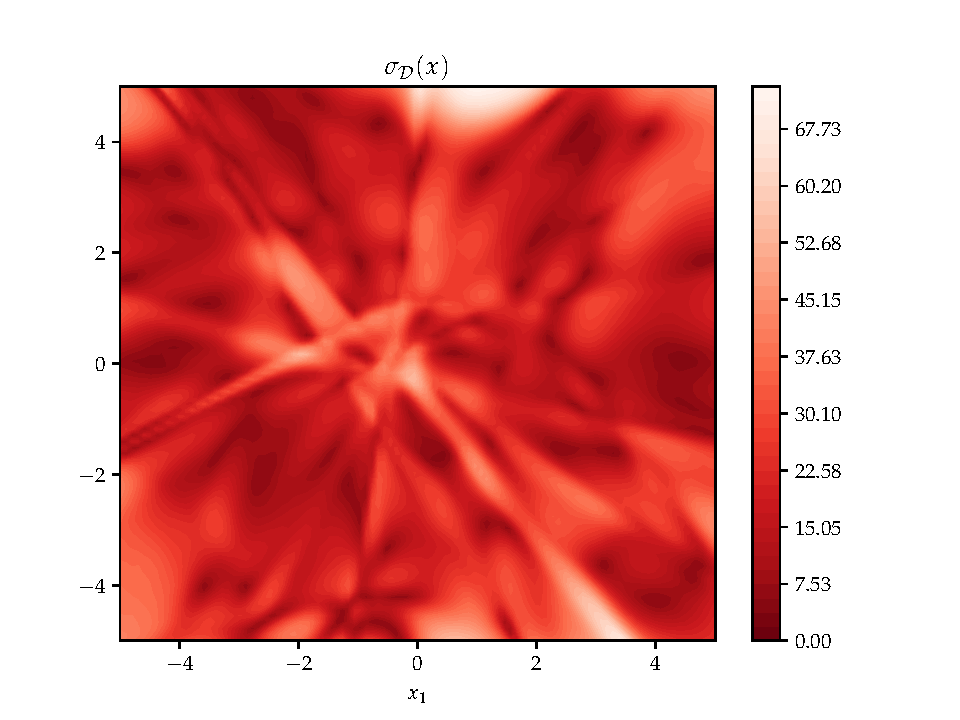
\includegraphics[trim=1.2cm 0.7cm 2cm 1cm,clip,width=\textwidth]{Figures/coco_reg/f23_numpyro neural network200-2003.pdf}
   \end{minipage}
  
   \begin{minipage}[b]{0.49\textwidth}
    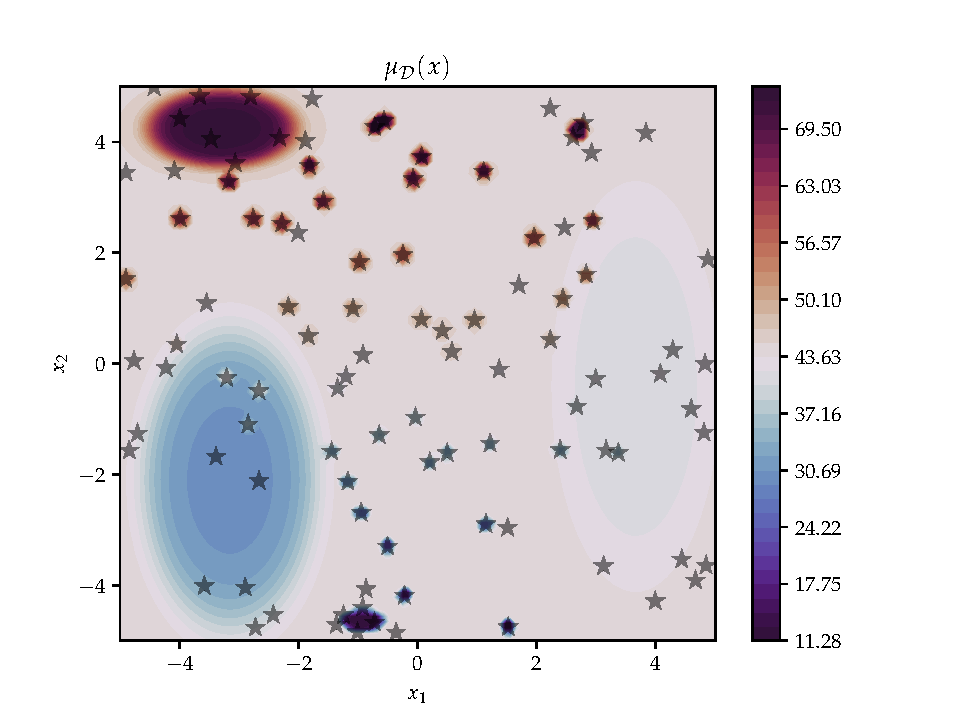
\includegraphics[trim=1.2cm 0.7cm 2cm 1cm,clip,width=\textwidth]{Figures/coco_reg/f23_SPN regression optimized2.pdf}
   \end{minipage}
   \hfill
   \begin{minipage}[b]{0.49\textwidth}
     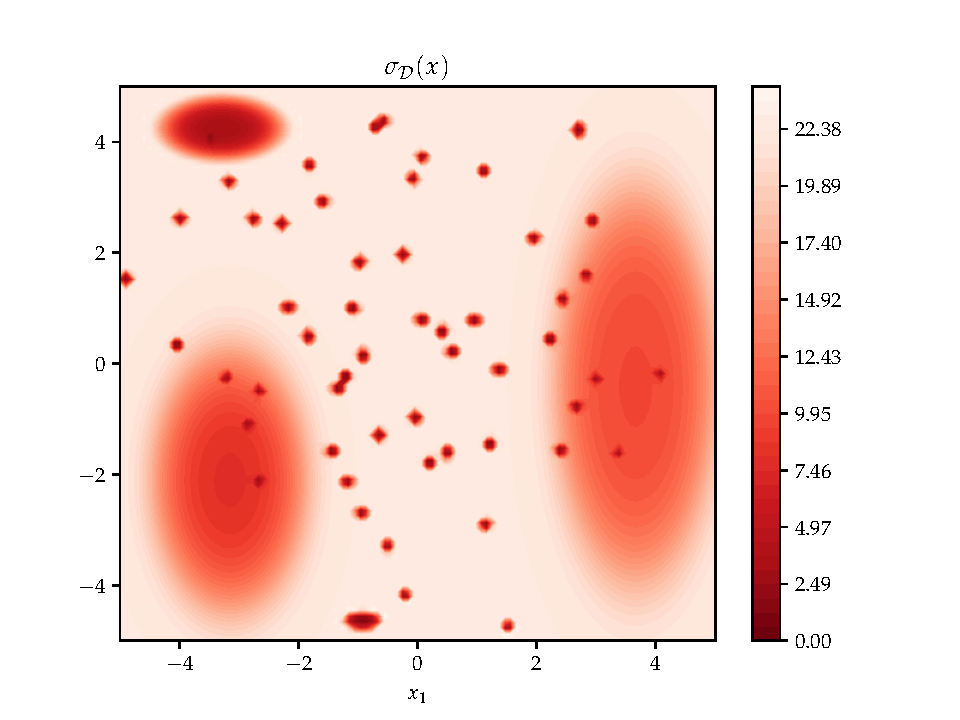
\includegraphics[trim=1.2cm 0.7cm 2cm 1cm,clip,width=\textwidth]{Figures/coco_reg/f23_SPN regression optimized3.pdf}
    \end{minipage}

    \begin{minipage}[b]{0.49\textwidth}
      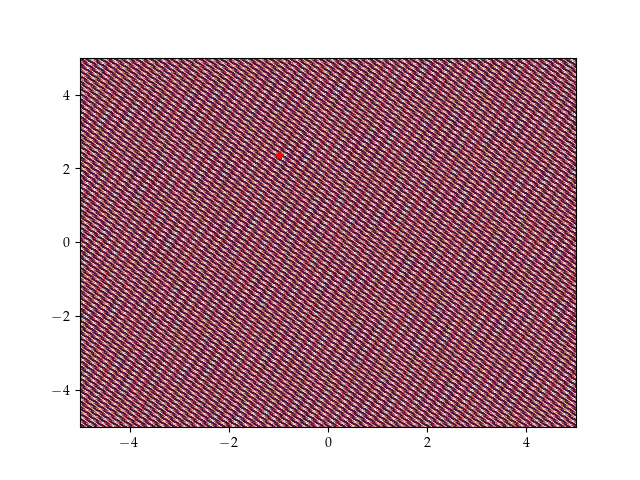
\includegraphics[trim=1.2cm 0.7cm 2cm 1cm,clip,width=\textwidth]{Figures/coco/f23.png}
     \end{minipage}
     \hfill
  \label{f1_reg_2D}
\end{figure}



\begin{figure}[h]
  \caption{2D Regression plot for a few of the problems, with the correct }
\end{figure}

\section{Mixture regression on simple functions}
Choosing a good set of design parameters is crucial, 
the manipulation... 

\begin{figure}[h]
    \caption{Regression plot for one problem with all dims: Number of data points / dims, mean squared error, with bayesline mean prediction}
\end{figure}

\begin{figure}[h]
    \caption{Regression plot for anther problem}
\end{figure}

% \begin{figure}[h]
%     \centering
%         \begin{tabular}{c|ll|l|l}
%         \multicolumn{1}{l|}{Problem 2D} & Winner (rel error)                                              & Second                                                                                  & Third                              &  \\ \cline{1-4}
%         f1                                                      & \multicolumn{1}{c|}{GP (0.2)}                                                           & \multicolumn{1}{c|}{\begin{tabular}[c]{@{}c@{}}Neural Network\\ (0.00001)\end{tabular}} & \multicolumn{1}{c|}{Naive (0.002)} &  \\
%         f2                                                      & \multicolumn{1}{c|}{Naive (0.002)}                                                      &                                                                                         &                                    &  \\
%         f3                                                      & \multicolumn{1}{c|}{\begin{tabular}[c]{@{}c@{}}Neural Network\\ (0.00001)\end{tabular}} &                                                                                         &                                    &  \\
%         f4                                                      & \multicolumn{1}{l|}{}                                                                   &                                                                                         &                                    &  \\
%                                                                 & \multicolumn{1}{l|}{}                                                                   &                                                                                         &                                    & 
%         \end{tabular}
%     \caption{Table summarizing for all problems}
% \end{figure}

\begin{figure}[h]
    \centering
    \begin{tabular}{llllll}
\hline
          & f1         & f2             & f3          & f4          & f5         \\
\hline
 BO\_numpy & 4.62(13.0) & 897.13(39.0)   & 2.07(36.0)  & 10.14(39.0) & 0.03(28.0) \\
 BO\_BOH   & 0.33(32.5) & 552.83(27.0)   & 5.51(33.0)  & 10.33(37.0) & 0.03(28.0) \\
 BO\_Gaus  & 0.89(8.0)  & 21.48(31.5)    & 21.86(21.0) & 16.32(25.5) & 0.03(22.5) \\
 BO\_Naiv  & 3.25(9.0)  & 72571.84(28.0) & 19.41(15.0) & 19.61(8.5)  & 4.35(21.0) \\
 BO\_em    & 1.23(24.5) & 455.28(10.0)   & 6.74(8.5)   & 5.98(30.5)  & 6.00(22.5) \\
\hline
\end{tabular}
    \caption{Distance to optima $f(x^{best})-f^*$ using Bayesian optimization with different surrogates
    and using expected improvement with a budget of $40$ samples for group 1: "5 separable functions"}
\end{figure}

\begin{figure}[h]
    \centering
    \begin{tabular}{lllll}
\hline
          & f6         & f7         & f8          & f9          \\
\hline
 BO\_numpy & 1.31(28.0) & 2.65(10.5) & nan(nan)    & nan(nan)    \\
 BO\_BOH   & 0.05(33.0) & 1.68(17.0) & 10.70(16.0) & 2.31(39.0)  \\
 BO\_Gaus  & 6.53(32.0) & 0.60(12.0) & 1.14(18.8)  & 0.27(25.0)  \\
 BO\_Naiv  & 4.74(20.0) & 4.71(25.5) & 11.87(2.0)  & 20.09(15.5) \\
 BO\_em    & 5.43(20.5) & 1.97(24.5) & 5.11(24.0)  & 68.97(8.0)  \\
\hline
\end{tabular}
    \caption{Distance to optima $f(x^{best})-f^*$ using Bayesian optimization with different surrogates
    and using expected improvement with a budget of $40$ samples for group 2: "4 functions with low or moderate conditioning"}
\end{figure}
\begin{figure}[h]
    \centering
    \begin{tabular}{llllll}
\hline
          & f10            & f11            & f12            & f13         & f14        \\
\hline
 BO\_numpy & nan(nan)       & nan(nan)       & nan(nan)       & nan(nan)    & nan(nan)   \\
 BO\_BOH   & 286.57(30.0)   & 7.48(35.0)     & 2770.49(31.0)  & 4.98(16.0)  & 0.03(30.0) \\
 BO\_Gaus  & 16.52(33.2)    & 638.31(32.0)   & 3033.71(27.8)  & 8.84(23.8)  & 0.01(36.5) \\
 BO\_Naiv  & 49166.58(27.0) & 2848.42(22.0)  & 23714.17(24.0) & 52.21(2.0)  & 0.61(31.0) \\
 BO\_em    & 61391.71(14.0) & 10317.74(20.5) & 673.63(12.5)   & 10.04(19.0) & 0.80(28.0) \\
\hline
\end{tabular}
    \caption{Distance to optima $f(x^{best})-f^*$ using Bayesian optimization with different surrogates
    and using expected improvement with a budget of $40$ samples for group 3: "5 functions with high conditioning, unimodal"}
\end{figure}
\begin{figure}[h]
    \centering
    \begin{tabular}{llllll}
\hline
          & f15         & f16         & f17        & f18         & f19         \\
\hline
 BO\_numpy & nan(nan)    & nan(nan)    & nan(nan)   & nan(nan)    & nan(nan)    \\
 BO\_BOH   & 10.05(20.0) & 9.02(33.0)  & 4.00(4.0)  & 3.55(38.0)  & 2.05(27.0)  \\
 BO\_Gaus  & 17.12(28.0) & 2.86(10.0)  & 3.15(18.5) & 3.26(10.0)  & 13.31(27.0) \\
 BO\_Naiv  & 34.09(20.5) & 3.20(20.5)  & 1.69(9.5)  & 11.72(24.0) & 3.36(5.0)   \\
 BO\_em    & 14.75(24.5) & 10.70(19.0) & 2.27(21.5) & 9.63(13.5)  & 1.99(9.5)   \\
\hline
\end{tabular}
    \caption{Distance to optima $f(x^{best})-f^*$ using Bayesian optimization with different surrogates
    and using expected improvement with a budget of $40$ samples for group 4: "5 multi-modal functions with adequate global structure"}
\end{figure}
\begin{figure}[h]
    \centering
    \begin{tabular}{llllll}
\hline
          & f20        & f21        & f22        & f23        & f24        \\
\hline
 BO\_numpy & nan(nan)   & nan(nan)   & nan(nan)   & nan(nan)   & nan(nan)   \\
 BO\_BOH   & 2.44(34.0) & 1.99(1.0)  & 1.98(25.0) & 2.64(15.0) & 8.98(14.0) \\
 BO\_Gaus  & 1.67(29.0) & 1.23(22.5) & 2.61(12.8) & 5.24(17.2) & 9.99(19.2) \\
 BO\_Naiv  & 2.43(15.5) & 0.27(21.5) & 2.04(4.0)  & 5.15(5.0)  & 7.15(26.5) \\
 BO\_em    & 3.16(17.0) & 1.07(15.0) & 0.90(22.0) & 5.66(13.5) & 3.82(6.5)  \\
\hline
\end{tabular}
    \caption{Distance to optima $f(x^{best})-f^*$ using Bayesian optimization with different surrogates
    and using expected improvement with a budget of $40$ samples for group 5: "5 multi-modal functions with weak global structure"}
\end{figure}

\begin{figure}[h]
    \centering
    \caption{BayesOpt plot: Number of iterations, distance to optima using EI, with bayesline random search}
\end{figure}


\begin{figure}[h]
    \centering
    \begin{minipage}[b]{0.32\textwidth}
     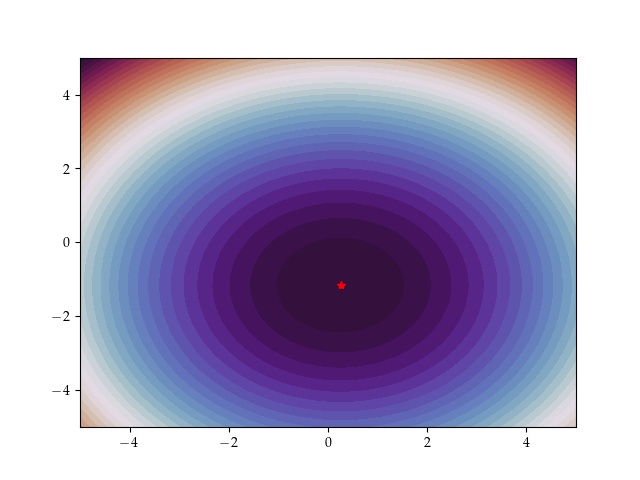
\includegraphics[trim=2.5cm 1.3cm 2.5cm 1.3cm,clip,width=\textwidth]{Figures/coco/f1.png}
    \end{minipage}
    \hfill
    \begin{minipage}[b]{0.32\textwidth}
     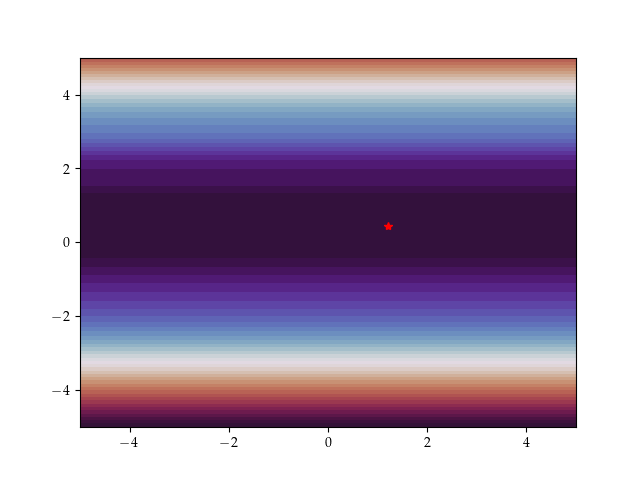
\includegraphics[trim=2.5cm 1.3cm 2.5cm 1.3cm,clip,width=\textwidth]{Figures/coco/f2.png}
    \end{minipage}
    \hfill
    \begin{minipage}[b]{0.32\textwidth}
      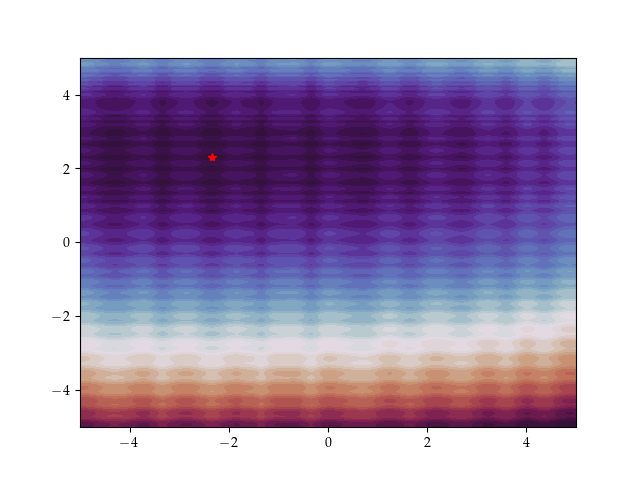
\includegraphics[trim=2.5cm 1.3cm 2.5cm 1.3cm,clip,width=\textwidth]{Figures/coco/f3.png}
      %\caption{Rank}
    \end{minipage}
    
    \begin{minipage}[b]{0.32\textwidth}
      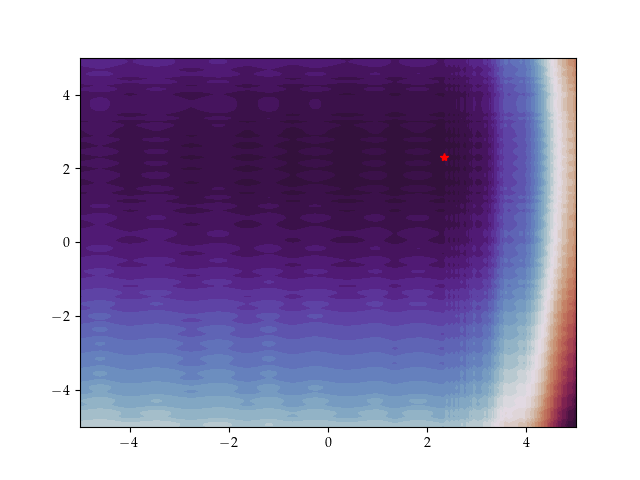
\includegraphics[trim=2.5cm 1.3cm 2.5cm 1.3cm,clip,width=\textwidth]{Figures/coco/f4.png}
    \end{minipage}
    \hfill
    \begin{minipage}[b]{0.32\textwidth}
      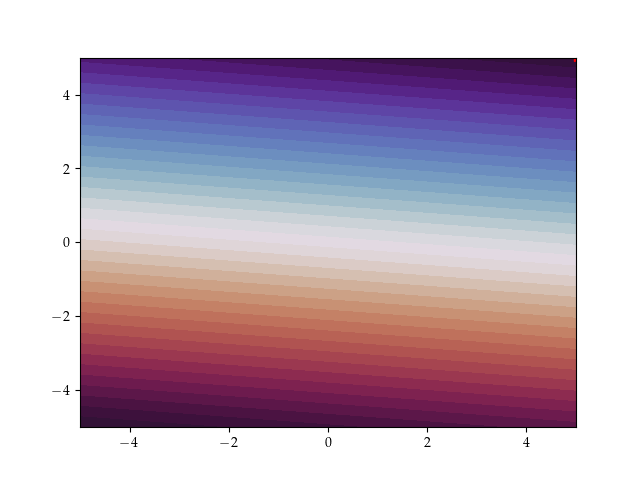
\includegraphics[trim=2.5cm 1.3cm 2.5cm 1.3cm,clip,width=\textwidth]{Figures/coco/f5.png}
    \end{minipage}
    \hfill
    \begin{minipage}[b]{0.32\textwidth}
      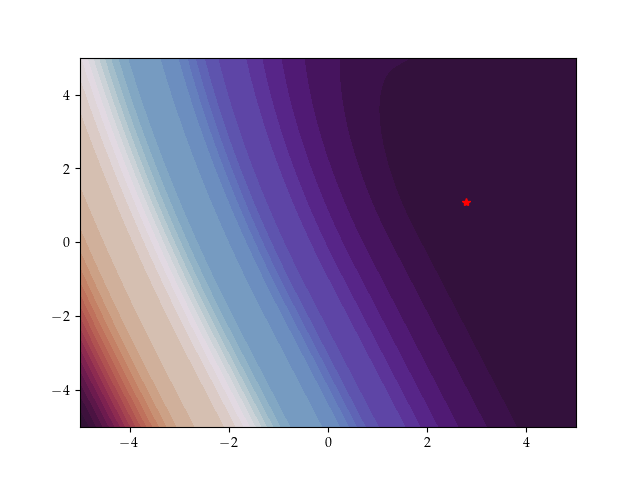
\includegraphics[trim=2.5cm 1.3cm 2.5cm 1.3cm,clip,width=\textwidth]{Figures/coco/f6.png}
    \end{minipage}
    

    \begin{minipage}[b]{0.32\textwidth}
      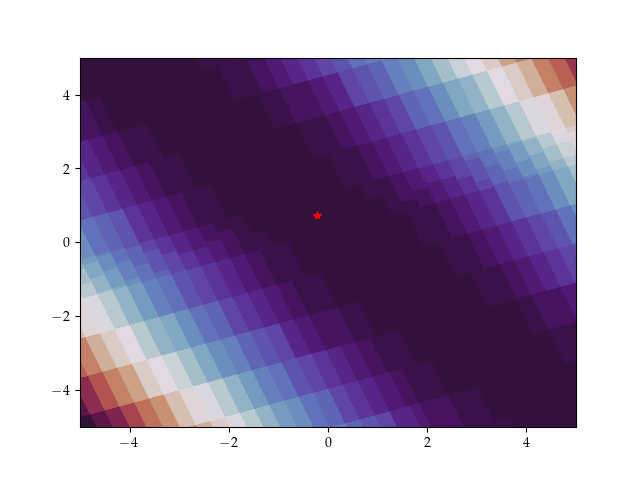
\includegraphics[trim=2.5cm 1.3cm 2.5cm 1.3cm,clip,width=\textwidth]{Figures/coco/f7.png}
    \end{minipage}
    \hfill
    \begin{minipage}[b]{0.32\textwidth}
      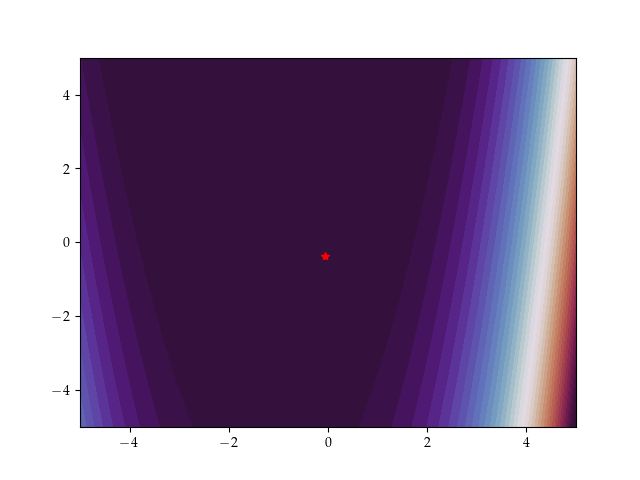
\includegraphics[trim=2.5cm 1.3cm 2.5cm 1.3cm,clip,width=\textwidth]{Figures/coco/f8.png}
    \end{minipage}
    \hfill
    \begin{minipage}[b]{0.32\textwidth}
      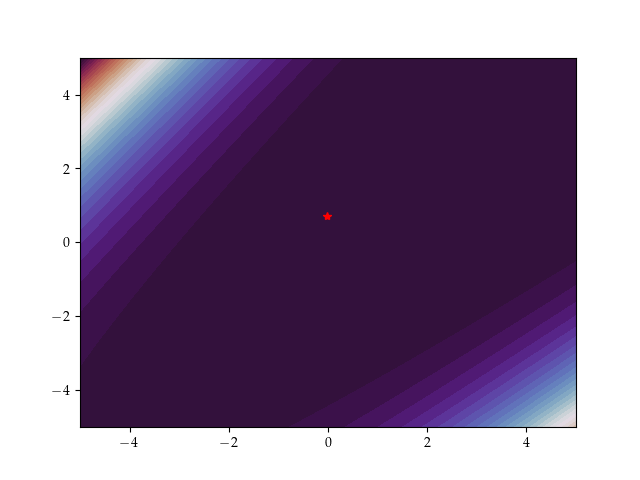
\includegraphics[trim=2.5cm 1.3cm 2.5cm 1.3cm,clip,width=\textwidth]{Figures/coco/f9.png}
    \end{minipage}
    
    \begin{minipage}[b]{0.32\textwidth}
        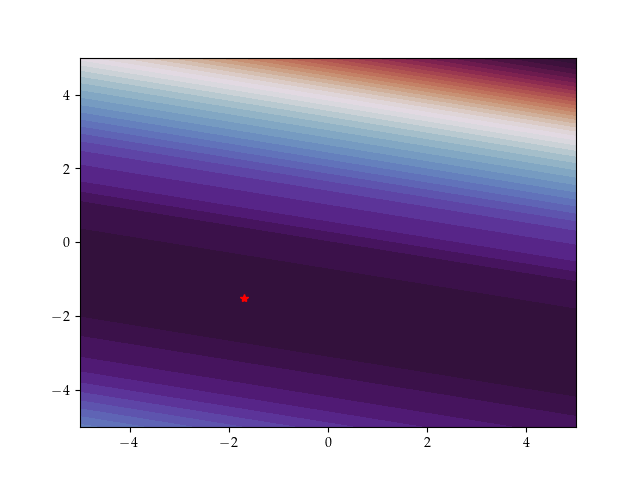
\includegraphics[trim=2.5cm 1.3cm 2.5cm 1.3cm,clip,width=\textwidth]{Figures/coco/f10.png}
    \end{minipage}
    \hfill
    \begin{minipage}[b]{0.32\textwidth}
      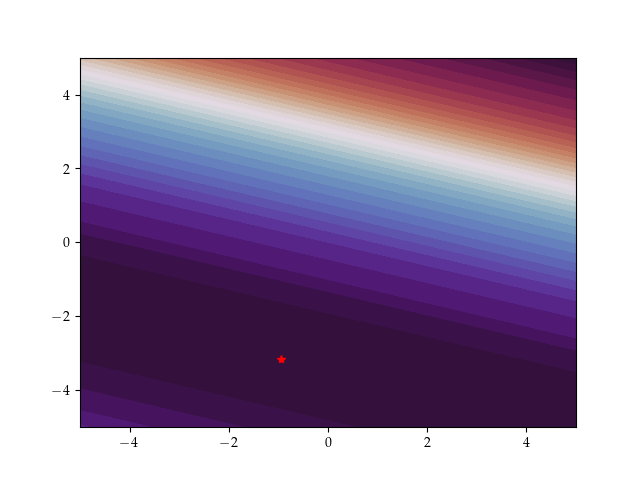
\includegraphics[trim=2.5cm 1.3cm 2.5cm 1.3cm,clip,width=\textwidth]{Figures/coco/f11.png}
    \end{minipage}
    \hfill
    \begin{minipage}[b]{0.32\textwidth}
      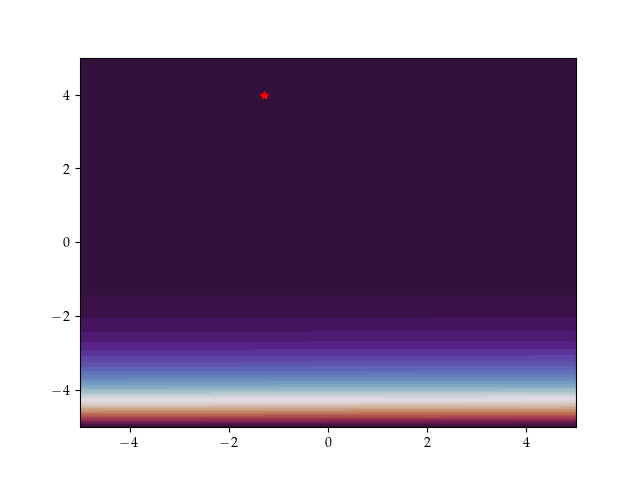
\includegraphics[trim=2.5cm 1.3cm 2.5cm 1.3cm,clip,width=\textwidth]{Figures/coco/f12.png}
    \end{minipage}
    \caption{Test functions f1 to f12}
    \label{2DBlockcyclic}
  \end{figure}
  
  \begin{figure}[h]
    \centering
    \begin{minipage}[b]{0.32\textwidth}
     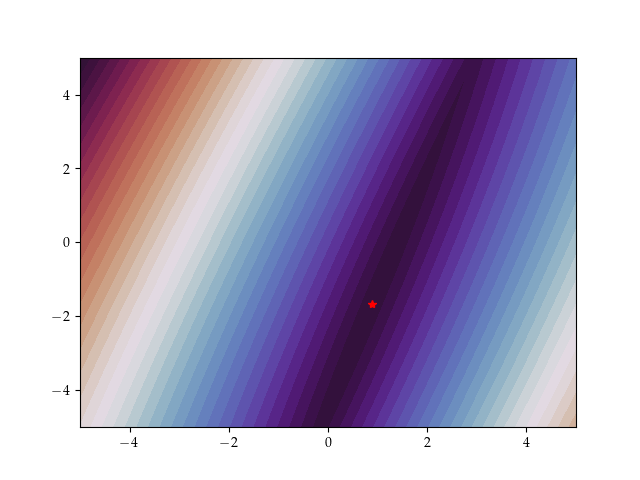
\includegraphics[trim=2.5cm 1.3cm 2.5cm 1.3cm,clip,width=\textwidth]{Figures/coco/f13.png}
    \end{minipage}
    \hfill
    \begin{minipage}[b]{0.32\textwidth}
     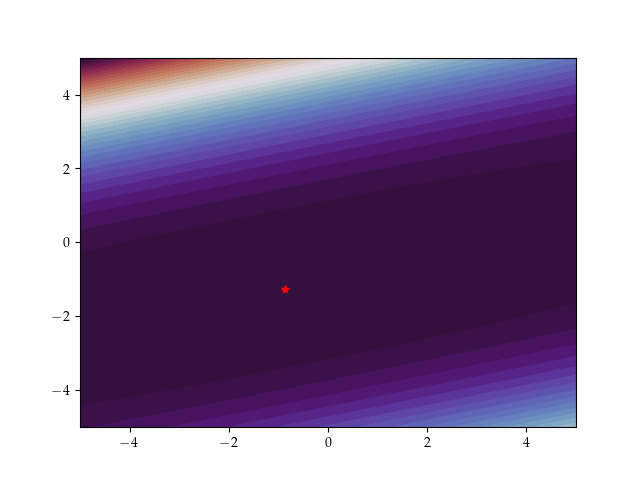
\includegraphics[trim=2.5cm 1.3cm 2.5cm 1.3cm,clip,width=\textwidth]{Figures/coco/f14.png}
    \end{minipage}
    \hfill
    \begin{minipage}[b]{0.32\textwidth}
      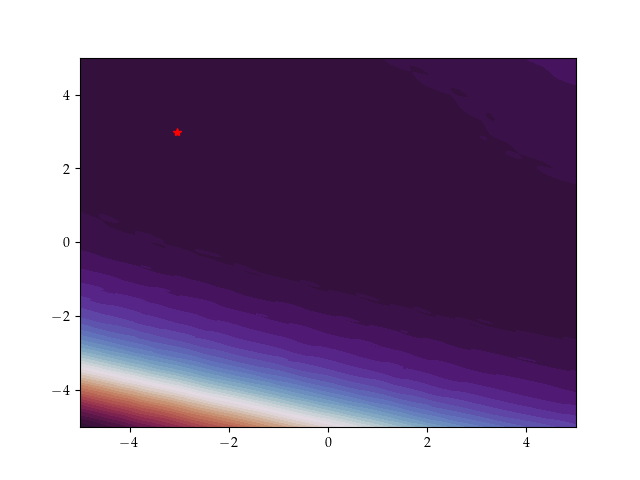
\includegraphics[trim=2.5cm 1.3cm 2.5cm 1.3cm,clip,width=\textwidth]{Figures/coco/f15.png}
      %\caption{Rank}
    \end{minipage}
    
    \begin{minipage}[b]{0.32\textwidth}
      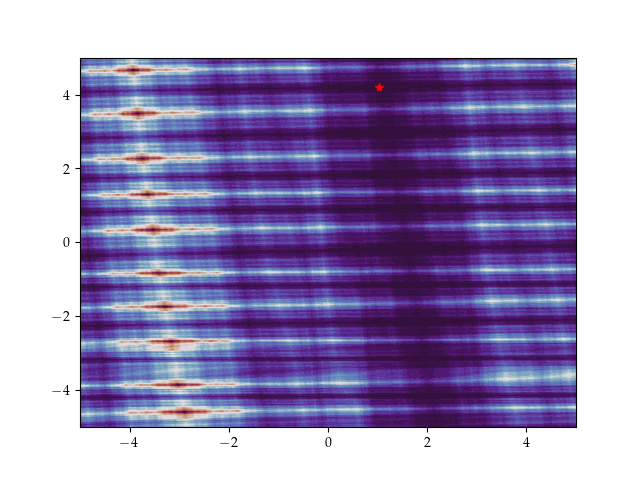
\includegraphics[trim=2.5cm 1.3cm 2.5cm 1.3cm,clip,width=\textwidth]{Figures/coco/f16.png}
    \end{minipage}
    \hfill
    \begin{minipage}[b]{0.32\textwidth}
      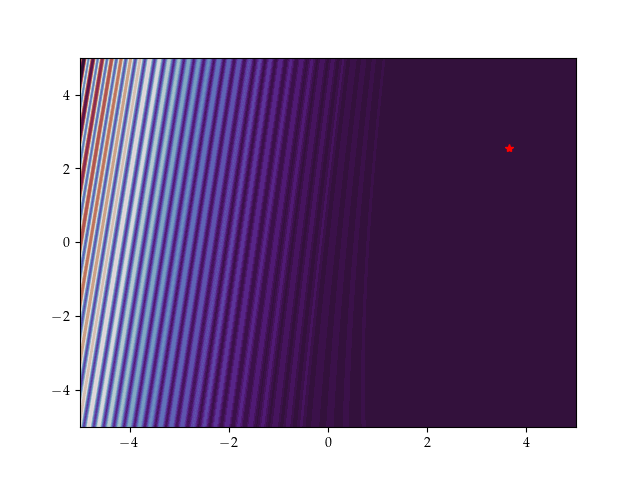
\includegraphics[trim=2.5cm 1.3cm 2.5cm 1.3cm,clip,width=\textwidth]{Figures/coco/f17.png}
    \end{minipage}
    \hfill
    \begin{minipage}[b]{0.32\textwidth}
      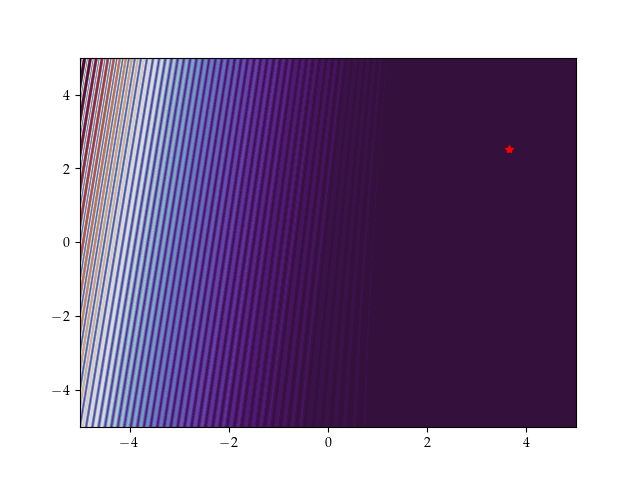
\includegraphics[trim=2.5cm 1.3cm 2.5cm 1.3cm,clip,width=\textwidth]{Figures/coco/f18.png}
    \end{minipage}
    

    \begin{minipage}[b]{0.32\textwidth}
      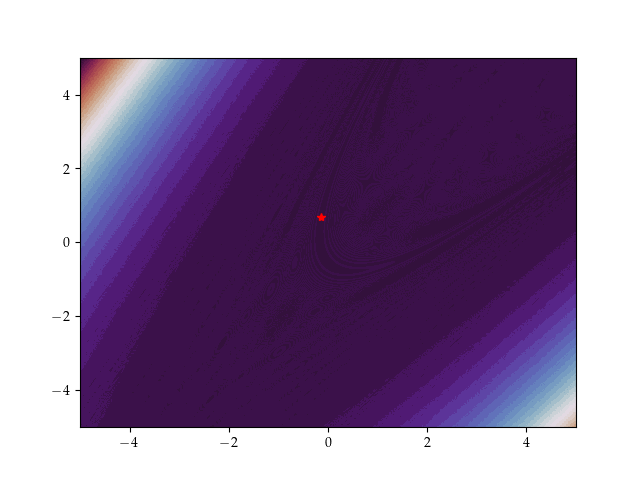
\includegraphics[trim=2.5cm 1.3cm 2.5cm 1.3cm,clip,width=\textwidth]{Figures/coco/f19.png}
    \end{minipage}
    \hfill
    \begin{minipage}[b]{0.32\textwidth}
      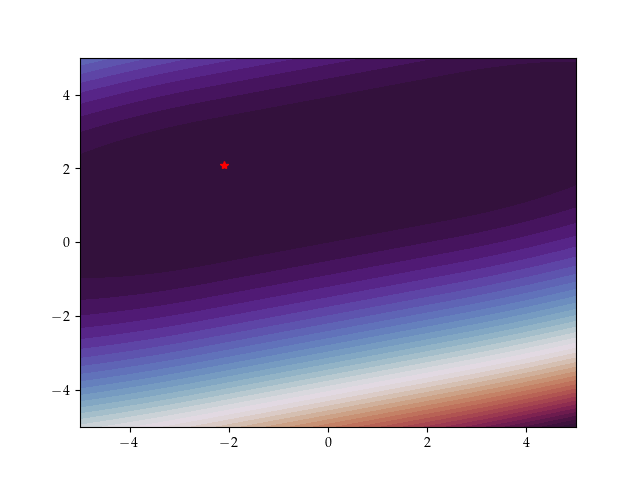
\includegraphics[trim=2.5cm 1.3cm 2.5cm 1.3cm,clip,width=\textwidth]{Figures/coco/f20.png}
    \end{minipage}
    \hfill
    \begin{minipage}[b]{0.32\textwidth}
      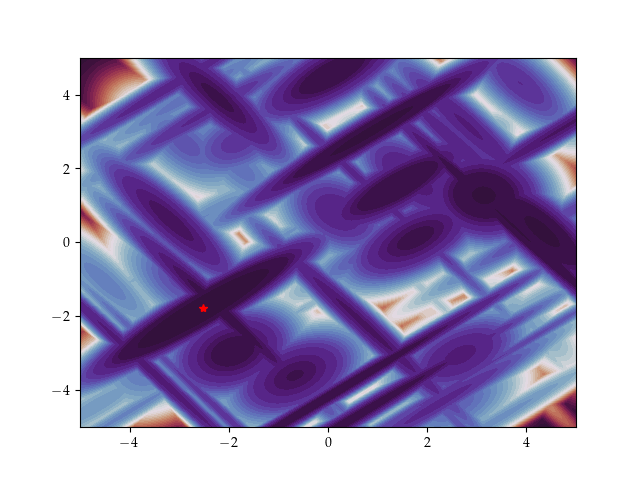
\includegraphics[trim=2.5cm 1.3cm 2.5cm 1.3cm,clip,width=\textwidth]{Figures/coco/f21.png}
    \end{minipage}
    
    \begin{minipage}[b]{0.32\textwidth}
        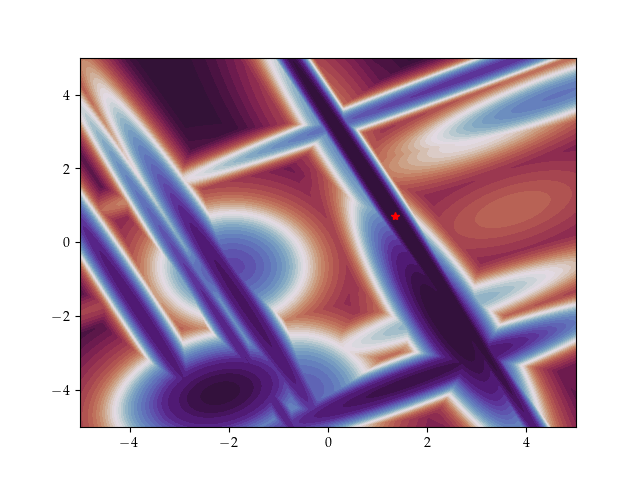
\includegraphics[trim=2.5cm 1.3cm 2.5cm 1.3cm,clip,width=\textwidth]{Figures/coco/f22.png}
    \end{minipage}
    \hfill
    \begin{minipage}[b]{0.32\textwidth}
      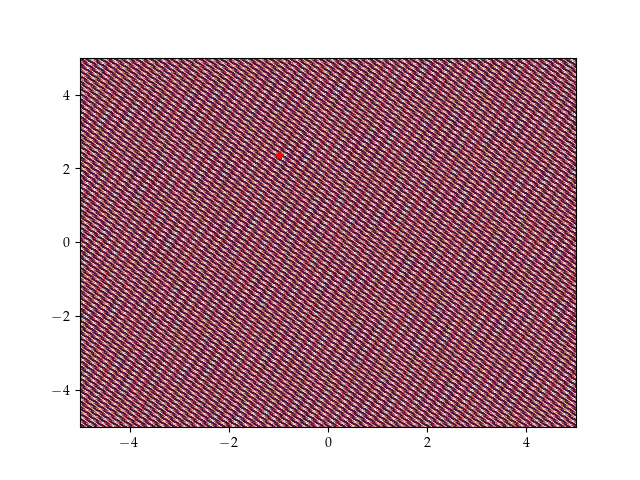
\includegraphics[trim=2.5cm 1.3cm 2.5cm 1.3cm,clip,width=\textwidth]{Figures/coco/f23.png}
    \end{minipage}
    \hfill
    \begin{minipage}[b]{0.32\textwidth}
      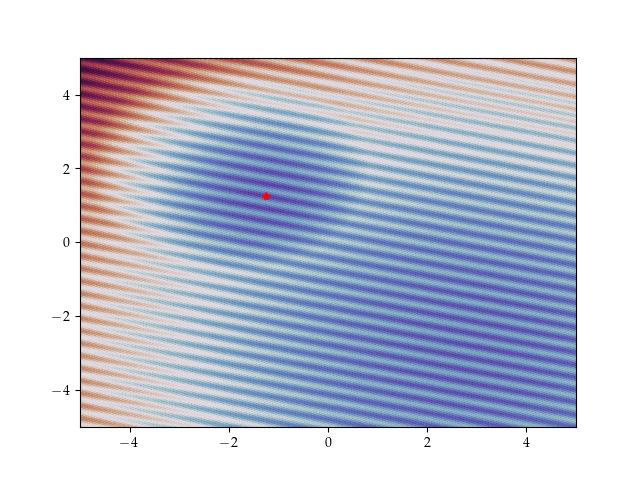
\includegraphics[trim=2.5cm 1.3cm 2.5cm 1.3cm,clip,width=\textwidth]{Figures/coco/f24.png}
    \end{minipage}
    \caption{Test functions f13-24}
    \label{f13-24}
  \end{figure}
  